\documentclass[11pt,a4paper]{article}
\usepackage{fontspec}
\usepackage[english]{babel}
\usepackage[margin=2.1cm]{geometry}
\usepackage{booktabs,array,tabularx}
\usepackage{xcolor}
\usepackage{graphicx}
\usepackage{pgfplots}
\pgfplotsset{compat=1.17}
\PassOptionsToPackage{hyphens}{url}
\usepackage[hidelinks]{hyperref}
\usepackage{enumitem}
\setlist{nosep,leftmargin=1.4em}
\emergencystretch=3em

\definecolor{impl}{HTML}{3B6EA8}
\definecolor{rev}{HTML}{8FB3DA}
\definecolor{waste}{HTML}{C8553D}

\title{Sweatshop on P-Chess: Audit fixes\\\large The d0920a0 audit's findings: save rollback (HIST-008), settings write failure (UI-038), cache validation (REV-010), History rebuild measurement (HIST-007), queue load repair (HIST-009) and dead code (CLEAN-015); GPT-6.1 Terra lineup, lane \texttt{audit-fixes}}
\author{Foreman, session \texttt{sweatshop/audit-fixes/2026-11-06-1433}}
\date{6 November 2026}

\begin{document}
\maketitle

\section*{Summary}

First run of the \texttt{audit-fixes} lane, on Windows, in a new clone at
\path{.artifacts-build/lanes/audit-fixes} made from \texttt{main} at \texttt{f6daf32}. That commit
holds the spec and the six tickets from Bruno's grill earlier the same day (two rounds through the
proxy: 14 questions settled by it, Q4 slicing and Q7 cache seam settled by Bruno). One launch at
14:33; the last merge was at 16:12, and the driver opened session PR
\href{https://github.com/Laginho/P-Chess/pull/43}{\#43}.

\begin{itemize}
  \item \textbf{Produced:} all six tickets merged on the session with \texttt{Verdict: Approve},
        all \texttt{Review: agent}, none reopened. One follow-up was filed during the run:
        HIST-010 (needs-triage, release impact), for the History rebuild stall that HIST-007
        measured.
  \item \textbf{Cost:} \textbf{\$6.07} at API list price over 12 stages, all priced:
        \texttt{gpt-6.1-terra xhigh} implementing \$2.02 (5), \texttt{gpt-6.1-sol xhigh}
        implementing the hard ticket \$0.71 (1), and \texttt{gpt-6.1-sol xhigh} reviewing \$3.34 (6).
        Codex quota: 4 points of the weekly window, from a 23\% baseline at 14:27, with no reset. Of
        those, Terra xhigh spent 3 and Sol xhigh 1 (1 implementing, 0 reviewing); one thread outside
        the stages spent 0. Each stage is $\pm$1 point, but the total is exact. Plan: the account's
        Codex plan.
  \item \textbf{What went wrong:} nothing in the loop. The product finding is that REV-010's
        validation made History's rebuild on each queue state change slower: about 450~ms on
        \texttt{main} rose to about 790~ms on the session, with 50 games. HIST-007 found the cost and
        the foreman confirmed it on both commits. It is now HIST-010.
  \item \textbf{Provisional verdict:} audit findings 2--6 are fixed and gated (569 passed,
        0 failed). Finding 1 is not closed: the per-event rebuild the audit measured is gone, but
        a rebuild of 0.8--0.9~s on each queue state change remains, and it is a release decision
        for Bruno.
\end{itemize}

\section*{What was done}

\textbf{HIST-008}: when saving a finished game fails at the stats file, the game no longer half
exists. The W/D/L, flag and practice counters are restored, and the PGN and repertoire snapshot
just written are deleted. The error names any file that could not be removed. A game whose
repertoire snapshot alone failed is still saved, as HIST-003 requires. Main file
\path{core/history.gd}. Not reopened.

\textbf{UI-038}: a setting that cannot be written is no longer reported as saved.
\texttt{Settings.set\_value} returns false, emits nothing and keeps the previous value. The name
dialog and Profile show the error inline, and the Settings screen controls snap back to the stored
value. \texttt{save\_last\_game} only warns in the log. Board resizing goes through
\texttt{changed}, so a failed save leaves the board where it was. Main files
\path{core/settings.gd}, \path{ui/settings.gd}, \path{ui/name_dialog.gd}, \path{ui/profile.gd}. Not
reopened.

\textbf{REV-010}: a saved analysis now counts as analysed only when it is complete. The check
covers the position count, each FEN against the game, the scores and the PV shape.
\texttt{Analyser.read\_analysis} takes the expected FENs and returns \texttt{stale} otherwise. Review,
History and Profile all read through it, and their own copies of the checks are gone. A corrupt
cache now shows the ``analyse again'' state instead of script errors. Main files
\path{engine/analyser.gd}, \path{ui/review.gd}, \path{ui/history_screen.gd}, \path{ui/profile.gd}.
Not reopened. Post-approval finding: computing the expected FENs for every History card
(\texttt{Analyser.positions\_from\_game}) added about 330--340~ms per rebuild (see Reopen
attribution).

\textbf{HIST-007}: History already kept parsed games between rebuilds, keyed by path and modified
time. Since Godot's modified time has whole-second resolution, the key now includes the file size,
and a game rewritten within the same second is reloaded. The measurement went over the 200~ms bar
in the spec: one rebuild with 50 games and 20 cards takes 0.8--0.9~s, and up to 1.6~s with older
PGNs that lack a \texttt{Reason} header. On the proxy's call, the cost was split by component and
filed as HIST-010 instead of widening the ticket. Main file \path{core/history.gd}. Not reopened.

\textbf{HIST-009}: a corrupt \path{analysis_queue.cfg} repairs itself on load. Non-string or empty
entries are dropped, a bad priority becomes empty and impossible counters are reset, with one
warning. The queue is never active without a game, so a valid game queued afterwards runs. Main
file \path{core/analysis_queue.gd}. Not reopened.

\textbf{CLEAN-015}: Review's unused \texttt{\_class\_help} and \texttt{\_wrap\_help} are deleted;
the legend on screen is unchanged. Main file \path{ui/review.gd}. Not reopened.

No roadmap image: P-Chess's \path{AGENTS.md} has no \texttt{Roadmap:} binding.

\section*{Timeline}

{\small
\begin{tabularx}{\linewidth}{@{}lX@{}}
\toprule
14:16--14:22 & Grill through the proxy (two rounds); spec and tickets committed and pushed to
        \texttt{main} (\texttt{f6daf32}). \\
14:33 & Clone made, dry run clean, driver launched (default lineup, Terra). Proxy ping answered. \\
14:34--14:48 & HIST-008 to review (10~min), merged (3~min). \\
14:48--15:08 & UI-038 to review (15~min), merged (5~min). \\
15:08--15:27 & REV-010 on the hard model (Sol xhigh), to review (14~min), merged (5~min). \\
15:27--15:48 & HIST-007 to review (16~min; proxy call at 15:31 opens HIST-010), merged (4~min). \\
15:48--16:01 & HIST-009 to review (9~min), merged (4~min). \\
16:02--16:12 & CLEAN-015 to review (7~min), merged (3~min). Nothing left; PR \#43. \\
16:20 & Foreman probe on \texttt{main} and on the session: History rebuild 438--460~ms against
        773--800~ms. \\
\bottomrule
\end{tabularx}
}

\section*{Per stage}

{\small
\begin{tabularx}{\linewidth}{@{}llllrrrrrX@{}}
\toprule
When & Ticket & Stage & Model & Min & In & Cache & Out & Cost & Outcome \\
\midrule
14:44 & HIST-008 & impl & terra xhigh & 10 & 4.9M & 98\% & 8k & 0.37 & to-review \\
14:48 & HIST-008 & review & sol xhigh & 3 & 1.8M & 93\% & 9k & 0.50 & merged \\
15:03 & UI-038 & impl & terra xhigh & 15 & 9.8M & 99\% & 12k & 0.63 & to-review \\
15:08 & UI-038 & review & sol xhigh & 5 & 2.4M & 94\% & 13k & 0.64 & merged \\
15:22 & REV-010 & impl & sol xhigh & 14 & 3.2M & 97\% & 22k & 0.71 & to-review \\
15:27 & REV-010 & review & sol xhigh & 5 & 2.6M & 94\% & 13k & 0.66 & merged \\
15:43 & HIST-007 & impl & terra xhigh & 16 & 6.8M & 99\% & 17k & 0.52 & to-review \\
15:48 & HIST-007 & review & sol xhigh & 4 & 1.7M & 91\% & 13k & 0.58 & merged \\
15:57 & HIST-009 & impl & terra xhigh & 9 & 4.6M & 99\% & 9k & 0.34 & to-review \\
16:01 & HIST-009 & review & sol xhigh & 4 & 2.3M & 95\% & 10k & 0.56 & merged \\
16:09 & CLEAN-015 & impl & terra xhigh & 7 & 1.8M & 97\% & 4k & 0.17 & to-review \\
16:12 & CLEAN-015 & review & sol xhigh & 3 & 1.2M & 91\% & 8k & 0.41 & merged \\
\midrule
 & & & & 95 & 43.1M & & 138k & 6.07 & \\
\bottomrule
\end{tabularx}
}

\begin{center}
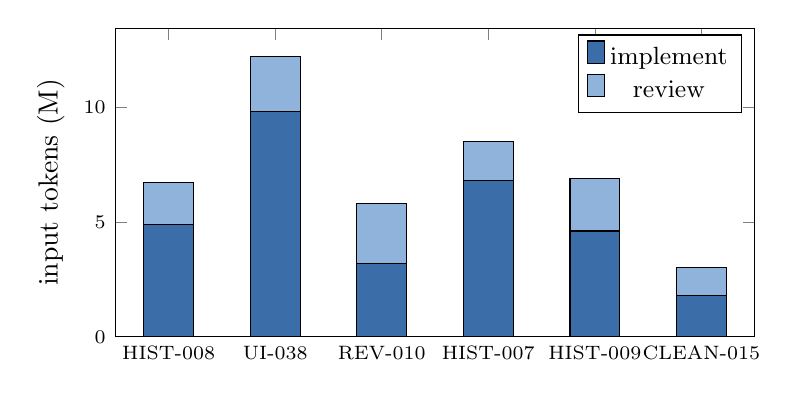
\begin{tikzpicture}
\begin{axis}[ybar stacked, bar width=18pt, width=0.8\linewidth, height=5.5cm,
  symbolic x coords={HIST-008,UI-038,REV-010,HIST-007,HIST-009,CLEAN-015},
  xtick=data, ylabel={input tokens (M)}, ymin=0, legend style={at={(0.98,0.98)},anchor=north east,font=\small},
  tick label style={font=\scriptsize}]
\addplot[fill=impl] coordinates {(HIST-008,4.9) (UI-038,9.8) (REV-010,3.2) (HIST-007,6.8) (HIST-009,4.6) (CLEAN-015,1.8)};
\addplot[fill=rev] coordinates {(HIST-008,1.8) (UI-038,2.4) (REV-010,2.6) (HIST-007,1.7) (HIST-009,2.3) (CLEAN-015,1.2)};
\legend{implement, review}
\end{axis}
\end{tikzpicture}
\end{center}

Wasted: nothing. No stage was lost, retried or reopened. UI-038 took the most input (9.8M): its
fix had to reach five callers. CLEAN-015, a 28-line deletion, still cost \$0.58 for its two stages.

\section*{Comparison with previous runs}

From \texttt{run-log.md}. \texttt{review-explore} (yesterday): \$11.40 for 3 (\$3.80 each), four
reopens, one lost stage. \texttt{qa-layout}: \$5.78 for 3 (\$1.93 each), one reopen. This run:
\$6.07 for 6 (\$1.01 each), no reopens, the cheapest run per ticket on P-Chess so far. Reviews cost
\$0.41--0.66 and took 3--5~min, against \$0.60--0.97 in \texttt{review-explore}. The tickets were
small, bounded fixes of findings that were already reproduced, with test seams set in the grill,
so this is not a like-for-like comparison with feature lanes.

\section*{Observations per model}

\begin{itemize}
  \item \textbf{gpt-6.1-terra xhigh, stage 2} (5 stages, 7--16~min): every ticket reached review
        on the first attempt, test-first, with red/green commit pairs. On HIST-007 it checked the
        measurement against a baseline copy of the previous \path{core/history.gd}. It noticed that
        its first estimate used an unrepresentative fixture, and asked the proxy instead of
        widening scope. Some of its PowerShell cleanup commands (\texttt{Remove-Item -Recurse}) were
        refused by Codex's policy; it worked around them.
  \item \textbf{gpt-6.1-sol xhigh, stage 2 (hard)} (REV-010): removed the three copies of the
        checks and added a type check on cached FENs after its own test caught one. The
        validation is correct, but it computes every card's positions on each History rebuild, a
        cost neither the ticket nor the review measured.
  \item \textbf{gpt-6.1-sol xhigh, review} (6 stages): zero findings in all six. It accepted
        HIST-008's snapshot-only path (criterion 4) by inspection, with no injected failure. On
        REV-010 it reviewed its own model's work, and it did not catch the History cost that
        HIST-007 measured 15 minutes later (review miss, below).
  \item \textbf{opus-5.5 xhigh, proxy}: two grill rounds before the run and one call during it
        (HIST-007). The call kept the ticket's scope and moved the design question to a new ticket,
        which is what the grill's rule asked for.
\end{itemize}

\section*{Driver and runtime issues}

\begin{enumerate}
  \item None. No crash, timeout, retry or API error. Shutdown 1.3--3.5~s per stage. Codex reached
        the proxy directly.
  \item The ticket text written by Codex on Windows turned en-dashes into \texttt{?} (HIST-007's
        Disclosure line, HIST-010). The meaning is still readable, but the encoding is lossy.
\end{enumerate}

\section*{Recommendations}

\begin{enumerate}
  \item Give any ticket that adds per-record work to a shared reader a criterion on the screens
        that call that reader in a loop. Here, History's cards: REV-010 passed every
        criterion and still slowed History down.
  \item Decide HIST-010 before tagging v0.1.0. \texttt{main} already exceeds the 200~ms bar
        (about 450~ms), and the session adds about 340~ms. Caching each card's derived data by path,
        modified time and size would remove both costs.
  \item Lineup: keep the default Terra lineup. Scoreboard rows: \texttt{gpt-6.1-terra xhigh
        $\rightarrow$ gpt-6.1-sol xhigh}, 41 reviews, 37\% reopened (S2 37\%), and
        \texttt{gpt-6.1-sol xhigh $\rightarrow$ gpt-6.1-sol xhigh}, 16 reviews, 19\% (S2 19\%). Both
        come from this machine's logs (see Scoreboard). This run's five Terra tickets and one Sol
        ticket all passed first time.
\end{enumerate}

\section*{Human debt and proxy decisions}

No \texttt{Débito humano:} lines in this run's tickets. All proxy decisions were made by
\texttt{opus-5.5 xhigh}; Codex reached the proxy directly.

\begin{itemize}
  \item All six tickets, grill round 1 (14:16): \texttt{Proxy decided (opus-5.5 xhigh): 9 settled,
        2 escalated}, with Q4 (slicing) and Q7 (where cache validation lives) sent to Bruno. Among
        the settled questions: finding 1 measured first, with a 200~ms bar; CLEAN-014 out of scope;
        rollback only on a stats-write failure; every \texttt{set\_value} caller re-shows the stored
        value; one session, \texttt{Review: agent}, no Windows manual acceptance; v0.1.0 tagged
        after the merge, with the push waiting for Bruno.
        (receipt \path{%TEMP%/sweatshop-proxy/20261106-141649-audit-fixes-c4b5e4.json})
  \item All six tickets, grill round 2 (14:21): \texttt{Proxy decided (opus-5.5 xhigh): 5 settled,
        0 escalated}. It settled the blocking order (HIST-007 after HIST-008 and REV-010, CLEAN-015
        after REV-010), the difficulty levels, the test seams (a directory in place of the target
        file, no timing assertion in the gate, size added to the cache key), the ticket shape and
        the launch. (receipt \path{%TEMP%/sweatshop-proxy/20261106-142124-audit-fixes-9f40af.json})
  \item HIST-007 (stage 2, 15:31): \texttt{Proxy decided (opus-5.5 xhigh)}: ``Hand off HIST-007
        with the cache-key fix as it stands. Don't widen Primary files or the test seam. Disclose
        the remaining $\sim$1.6~s stall as deferred with release impact, and open a needs-triage
        follow-up for it. The numbered criteria are already met, and the real cost sits in a
        design choice the grill never settled.''
        (receipt \path{%TEMP%/sweatshop-proxy/20261106-153131-HIST-007-718613.json})
\end{itemize}

\section*{Acceptance}

The spec has no acceptance scenarios. Its acceptance is each ticket's numbered criteria on the
agreed automated seams (grill Q9), and no Windows manual check. The gate on the integrated session
head (CLEAN-015's) passed with 569 tests and 0 failures; six real-Lc0 checks and one pixel check
were skipped. The foreman added one observable probe, History's rebuild on \texttt{main} against the
session (three runs each, headless, 50 finished 40-ply games, 20 cards, rendering excluded):
438/460/450~ms against 773/792/800~ms. Product acceptance by ticket, as recorded in PR \#43:
\begin{itemize}
  \item Passed: HIST-008, REV-010, HIST-009 and CLEAN-015.
  \item Pending, with no hold: UI-038, whose graphical look of the inline errors is unexamined.
  \item Pending, with release impact: HIST-007, which remains open through HIST-010.
\end{itemize}
Not examined: real disk-full or permission errors on Windows, a graphical look at the error text,
and real Stockfish caches.

\section*{Reopen attribution}

No reopens and no fixes made during review in this run. One post-approval finding, labelled by
the foreman (opus-5.5; the implementer and the reviewer were both \texttt{gpt-6.1-sol xhigh}, so
this is not self-judging). The row is appended to \path{.scratch/reopen-attribution.md}.

{\small\noindent
\begin{tabularx}{\linewidth}{@{}>{\raggedright\arraybackslash}p{1.7cm}X>{\raggedright\arraybackslash}p{2.3cm}X@{}}
\toprule
Ticket (round) & Finding & Label & Why \\
\midrule
REV-010 (-) & History rebuild went from $\sim$450 to $\sim$790~ms; every card now computes its positions for \texttt{read\_analysis} & S2-implícito ? & a regression of its own change, reachable from the ticket and the code; no criterion named it. Discovery \texttt{session-review}; review miss yes; churn no \\
\bottomrule
\end{tabularx}
}

Totals for this run: S2-implícito 1 (borderline, post-approval). No S1, S2-explícito or S3. Release
audit findings 2--6 (recorded on 5 November as \texttt{release-audit}) are fixed by HIST-008,
UI-038, REV-010 and HIST-009. Finding 1 continues in HIST-010.

\section*{Scoreboard}

\texttt{scoreboard.ps1} over this Windows machine's main checkouts: ClassyCall, EasyMath, P-Chess
(with this run's rows, attribution and interventions merged), PhysiSyst, SIGAA-ME and SynchroNice.
The previous report's scoreboard ran on the Linux box, whose logs hold more runs (EasyMath's lanes,
\texttt{slip}), so most rows are smaller here and are \textbf{not} comparable with that report. The
only rows this run moved are \texttt{gpt-6.1-terra xhigh} and \texttt{gpt-6.1-sol xhigh} as
implementers, five and one more stages to review with none failed, and the pairs below with no new
reopens. Interventions: proxy-decision (opus-5.5 xhigh) rose by 3.

{\tiny
\begin{verbatim}
| Implementer | Stage runs | To review | Failed | Asked | Median min to review | Cost |
|---|---|---|---|---|---|---|
| gpt-6.1-sol high | 68 | 63 | 0 | 5 | 9m | $47.66 (68/68 priced) |
| opus-5.5 xhigh | 18 | 14 | 4 | 0 | 12m | $91.78 (18/18 priced) |
| gpt-6.1-sol max | 6 | 5 | 0 | 1 | 24m | $12.12 (6/6 priced) |
| opus-5.5 high | 20 | 13 | 6 | 1 | 6m | $37.46 (20/20 priced) |
| gpt-6.1-sol xhigh | 16 | 16 | 0 | 0 | 13m | $12.84 (16/16 priced) |
| gpt-6.1-terra high | 32 | 20 | 10 | 2 | 7m | $8.54 (32/32 priced) |
| gpt-6.1-terra xhigh | 51 | 42 | 8 | 1 | 10m | $34.67 (51/51 priced) |
(other implementer rows omitted: models outside this lineup)

| Implementer | Reviewer | Reviews | Reopened | Reopen rate | Reopened for S2 | S2 rate | Unclassified | Fixed in review for S2 |
|---|---|---|---|---|---|---|---|---|
| gpt-6.1-sol high | gpt-6.1-sol xhigh | 22 | 5 | 23% | 5 | 23% | 0 | 0 |
| gpt-6.1-sol xhigh | gpt-6.1-sol xhigh | 16 | 3 | 19% | 3 | 19% | 0 | 1 |
| gpt-6.1-terra high | gpt-6.1-sol xhigh | 20 | 6 | 30% | 6 | 30% | 0 | 0 |
| ? | gpt-6.1-sol xhigh | 4 | 1 | 25% | 0 | 0% | 0 | 0 |
| gpt-6.1-terra xhigh | gpt-6.1-sol xhigh | 41 | 15 | 37% | 15 | 37% | 0 | 3 |
(pairs under other reviewers omitted)

| Implementer -> Reviewer | Rounds | S2 explicit code | S2 explicit test | S2 implicit | S1 | S3 noise |
|---|---|---|---|---|---|---|
| gpt-6.1-sol xhigh -> gpt-6.1-sol xhigh | 6 | 6 | 0 | 3 | 0 | 0 |
| gpt-6.1-terra high -> gpt-6.1-sol xhigh | 9 | 10 | 1 | 3 | 1 | 0 |
| gpt-6.1-terra xhigh -> gpt-6.1-sol xhigh | 42 | 52 | 2 | 13 | 5 | 0 |

| Discovery | Recorded findings | Earlier review miss (yes / known) | Review-induced churn (yes / known) |
|---|---|---|---|
| ticket-review | 456 | 9 / 261 | 1 / 263 |
| session-review | 37 | 30 / 32 | 0 / 32 |
| release-audit | 7 | 2 / 2 | 0 / 2 |
Runtime completion to process exit: 436.001s total over 344 measured stages; 334 unmeasured.
| Intervention | Recorded events |
|---|---|
| human-rescue | 33 |
| automatic-recovery | 130 |
| proxy-decision (unknown) | 37 |
| routine-approval | 19 |
| proxy-decision (gpt-6-astra high, fallback) | 58 |
| proxy-decision (opus) | 42 |
| proxy-decision (supervisor) | 12 |
| proxy-decision (opus-5.5 xhigh) | 53 |
\end{verbatim}
}

Under the same reviewer (Sol xhigh), Terra xhigh (41 reviews) reopens more often than Sol xhigh
(16) and Terra high (20). The Sol xhigh pair sees only hard or escalated tickets, so the
comparison is not like for like, and 16 reviews is close to anecdote.

\section*{Pending for the human}

\begin{enumerate}
  \item Decide HIST-010 (History rebuild 0.8--0.9~s on each queue state change, about 340~ms of it
        from REV-010; \texttt{main} is already about 450~ms): fix it before v0.1.0, or tag with it as
        known debt.
  \item Review and merge PR \#43.
  \item After the merge, give the go to push the \texttt{v0.1.0} tag.
  \item Optionally: HIST-008's snapshot-only failure path has no injected test (accepted by
        inspection), and CLEAN-014 is still in triage.
\end{enumerate}

\end{document}
